\documentclass[tikz,border=2pt]{standalone}
\usepackage{amsmath,amssymb}
\usepackage{tikz}

\begin{document}
% Convex: the segment between any two points stays inside. Not convex: some segment leaves
% the set (the kidney shape has a dent).
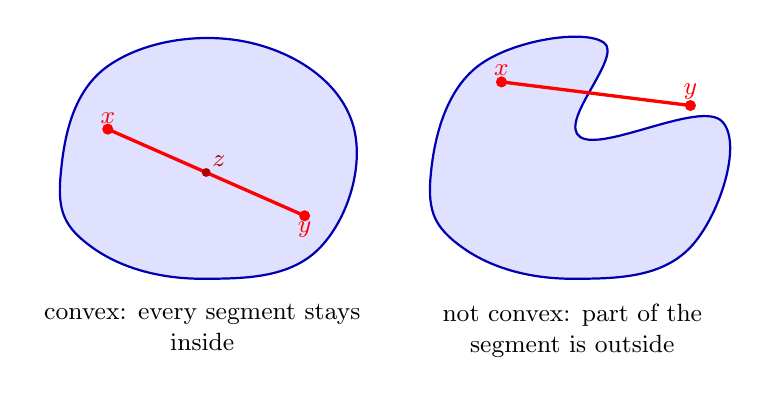
\begin{tikzpicture}[every node/.style={font=\small}]
	\begin{scope}
		\fill[blue!12] plot[smooth cycle, tension=0.7] coordinates {(-1.8,-0.2) (-1.2,1.2) (0.6,1.5) (1.9,0.5) (1.5,-1.1) (0,-1.5) (-1.4,-1.1)};
		\draw[blue!70!black, thick] plot[smooth cycle, tension=0.7] coordinates {(-1.8,-0.2) (-1.2,1.2) (0.6,1.5) (1.9,0.5) (1.5,-1.1) (0,-1.5) (-1.4,-1.1)};
		\draw[red, very thick] (-1.2,0.4) -- (1.3,-0.7);
		\fill[red] (-1.2,0.4) circle (2pt) node[above, inner sep=2pt] {$x$};
		\fill[red] (1.3,-0.7) circle (2pt) node[below, inner sep=2pt] {$y$};
		\fill[red!70!black] (0.05,-0.15) circle (1.6pt) node[above right, inner sep=2pt] {$z$};
		\node[anchor=north, align=flush center, text width=4.2cm] at (0,-1.7) {convex: every segment stays inside};
	\end{scope}
	\begin{scope}[xshift=4.7cm]
		\fill[blue!12] plot[smooth cycle, tension=0.7] coordinates {(-1.8,-0.2) (-1.2,1.2) (0.4,1.5) (0.1,0.3) (1.9,0.5) (1.5,-1.1) (0,-1.5) (-1.4,-1.1)};
		\draw[blue!70!black, thick] plot[smooth cycle, tension=0.7] coordinates {(-1.8,-0.2) (-1.2,1.2) (0.4,1.5) (0.1,0.3) (1.9,0.5) (1.5,-1.1) (0,-1.5) (-1.4,-1.1)};
		\draw[red, very thick] (-0.9,1.0) -- (1.5,0.7);
		\fill[red] (-0.9,1.0) circle (2pt) node[above, inner sep=2pt] {$x$};
		\fill[red] (1.5,0.7) circle (2pt) node[above, inner sep=2pt] {$y$};
		\node[anchor=north, align=flush center, text width=4.2cm] at (0,-1.7) {not convex: part of the segment is outside};
	\end{scope}
\end{tikzpicture}
\end{document}
